\documentclass[a4paper, 12pt]{article}
\usepackage[utf8]{inputenc}
\usepackage[italian]{babel}
\usepackage{imakeidx}
\usepackage{graphicx}
\usepackage{titlesec}
\usepackage{verbatim}
\usepackage{amsmath}
\usepackage{amssymb}
\usepackage{listings}
\usepackage{parskip}
\usepackage{wrapfig}
\usepackage{tabu}

% Custom margins
\usepackage[a4paper, inner=1cm, outer=2.7cm, top=1.1cm, bottom=3cm, bindingoffset=1.2cm]{geometry}

% List spacing
\usepackage{enumitem}
\setlist{topsep=2pt, itemsep=2pt, partopsep=2pt, parsep=2pt}

% Header and footer
\usepackage{fancyhdr}
\pagestyle{fancy}
\fancyhf{}
\lhead{Prova Finale - Reti Logiche - A.A. 2020/2021}
\rhead{Alberto Pirillo}
\renewcommand{\footrulewidth}{0.4pt}
\cfoot{\thepage}

% Title 
\title{\Huge{Prova Finale - Reti Logiche}}
\author{\Large{Alberto Pirillo - 10667220} \\ \Large{Prof. Gianluca Palermo}}
\date{Anno Accademico 2020/2021}

\makeindex
\begin{document}
\maketitle
\tableofcontents
\newgeometry{inner=1cm, outer=2.7cm, top=3cm, bottom=3cm, bindingoffset=1.2cm}
\pagebreak

\section{Introduzione}
\subsection{Scopo del progetto}
Lo scopo del progetto è quello di utilizzare il tool \textit{Xilinx Vivado WebPack} per  descrivere in VHDL e sintetizzare un componente HW in grado di:
\begin{itemize}
    \item Leggere un'immagine interfacciandosi con una memoria
    \item Processare l'immagine con un algoritmo di equalizzazione dell'istogramma
    \item Salvare il risultato finale in tale memoria
\end{itemize}

\subsection{Specifiche generali}
L'obiettivo del metodo di equalizzazione dell'istogramma di un'immagine è quello di ricalibrare il contrasto di un'immagine quando l'intervallo dei valori di intensità è molto ridotto, in modo da incrementare il contrasto. Viene applicata una versione semplificata dell'algoritmo, descritta di seguito.

\bigskip\footnotesize
$DELTA\_VALUE = MAX\_PIXEL\_VALUE - MIN\_PIXEL\_VALUE$ \\
$SHIFT\_LEVEL = (8-FLOOR(LOG_2(DELTA\_VALUE + 1)))$ \\
$TEMP\_PIXEL = (CURRENT\_PIXEL\_VALUE - MIN\_PIXEL\_VALUE) \ll SHIFT\_LEVEL$ \\
$NEW\_PIXEL\_VALUE = MIN(255, TEMP\_PIXEL)$
\bigskip\normalsize

\begin{itemize}
    \item MAX\_PIXEL\_VALUE è il massimo valore dei pixel dell'immagine
    \item MIN\_PIXEL\_VALUE è il minimo valore dei pixel dell'immagine
    \item CURRENT\_PIXEL\_VALUE è il valore del pixel da equalizzare 
    \item NEW\_PIXEL\_VALUE è il valore del pixel equalizzato
\end{itemize}

\bigskip
Ogni immagine è in scala di grigi e ha una dimensione compresa tra 1x1 e 128x128 pixel. Ogni pixel può assumere un valore compreso tra 0 e 255. \\
Il dispositivo è in grado anche di gestire un'immagine "nulla", ossia con una o entrambe le dimensioni formate da 0 pixel.
\\\\
L'immagine è memorizzata in modo contiguo in memoria e il dispositivo da implementare dovrà leggerla sequenzialmente e riga per riga. L'immagine equalizzata deve essere scritta in memoria nella posizione immediatamente successiva a quella occupata dall'originale.

\subsection{Struttura della memoria}
L'immagine è memorizzata in una memoria con indirizzamento al byte partendo dalla posizione 0.
Si assume che tale memoria sia già instanziata e dunque non debba essere sintetizzata.
Inoltre, ogni pixel dell'immagine è memorizzato con codifica binaria su 8 bit senza segno.
\bigskip
\begin{itemize}
    \item Il byte in posizione 0 si riferisce al numero di colonne dell'immagine
    \item Il byte in posizione 1 si riferisce al numero di righe dell'immagine
    \item I pixel dell'immagine sono memorizzati in memoria partendo dal byte in posizione 2
    \item I pixel dell'immagine equalizzata devono essere memorizzati in memoria partendo dal byte in posizione immediatamente successiva all'ultimo pixel dell'immagine originale
\end{itemize}

\begin{figure}[h]
    \centering
    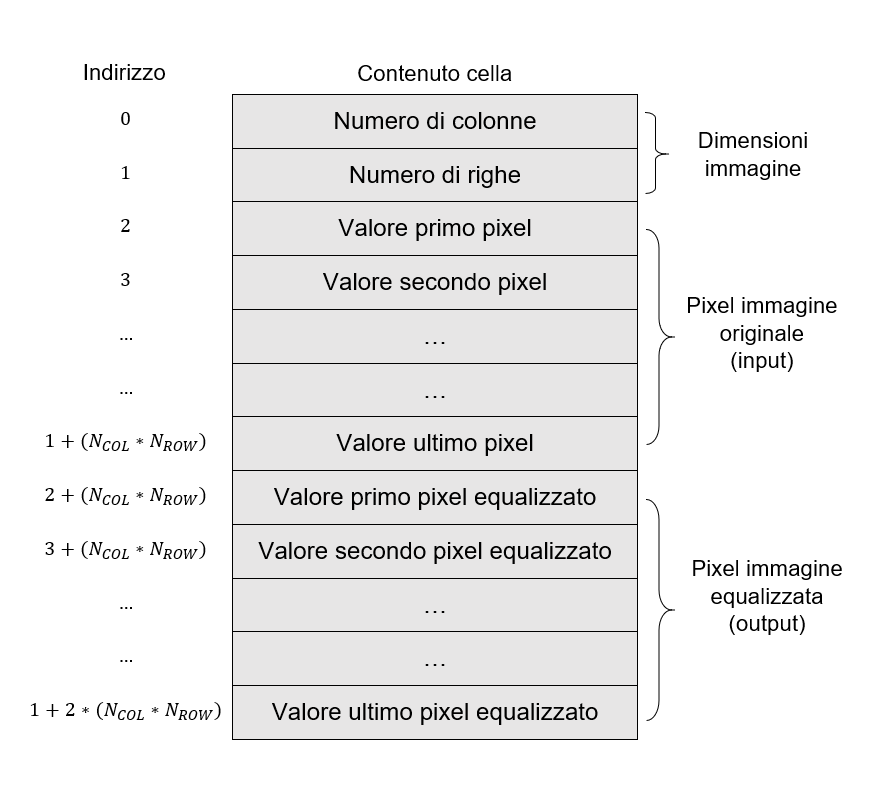
\includegraphics[scale=0.90]{introduzione/memory_scheme.png}
    \caption{Schema del contenuto delle celle di memoria, con i rispettivi indirizzi}
    \label{fig:memory_scheme}
\end{figure}

\newpage
\subsection{Funzionamento della memoria}
La memoria utilizzata consiste in una Single-Port Block RAM Write-First-Mode.

La sua interfaccia è la seguente:
\begin{lstlisting}[language=VHDL]
entity rams_sp_wf is
    port(
        clk  : in std_logic;
        we   : in std_logic;
        en   : in std_logic;
        addr : in std_logic_vector(15 downto 0);
        di   : in std_logic_vector(7 downto 0);
        do   : out std_logic_vector(7 downto 0)
    );
end rams_sp_wf;
\end{lstlisting}

\bigskip
In breve, il funzionamento della memoria richiede che \textbf{en} = 1 per effettuare qualunque operazione (sia lettura che scrittura). 

Inoltre, a ogni ciclo di clock, viene letto il valore di \textbf{addr}:

\begin{itemize}
    \item se \textbf{we} = 1: viene copiato \textbf{di} nella cella di memoria con indirizzo corrispondente al valore di \textbf{addr}
    \item se \textbf{we} = 0: viene copiato in \textbf{do} il valore contenuto nella cella di memoria con indirizzo corrispondente al valore di \textbf{addr}
\end{itemize}

\bigskip
In entrambi i casi, tali valori sono disponibili al ciclo di clock successivo.


\newpage
\section{Architettura}
\subsection{Interfaccia del componente}
Il componente implementato presenta la seguente interfaccia:

\begin{lstlisting}[language=VHDL]
entity project_reti_logiche is
    port (
        i_clk     : in std_logic;
        i_rst     : in std_logic;
        i_start   : in std_logic;
        i_data    : in std_logic_vector(7 downto 0);
        o_address : out std_logic_vector(15 downto 0);
        o_done    : out std_logic;
        o_en      : out std_logic;
        o_we      : out std_logic;
        o_data    : out std_logic_vector (7 downto 0)
    );
end project_reti_logiche;
\end{lstlisting}

\begin{itemize}
    \item \textbf{i\_clk:} segnale di CLOCK in ingresso generato dal TestBench
    \item \textbf{i\_rst:} segnale di RESET che inizializza la macchina, in modo che sia pronta per ricevere il primo segnale di START
    \item \textbf{i\_start:} segnale di START generato dal TestBench
    \item \textbf{i\_data:} segnale (vettore) che arriva dalla memoria in seguito a una richiesta di lettura
    \item \textbf{o\_address:} segnale (vettore) di uscita che determina l’indirizzo della memoria su cui effettuare un'operazione
    \item \textbf{o\_done:} segnale di uscita che comunica la fine dell’elaborazione e la completa scrittura del dato in memoria
    \item \textbf{o\_en:} segnale di ENABLE richiesto dalla memoria per poter comunicare, sia in lettura che in scrittura
    \item \textbf{o\_we:} segnale di WRITE ENABLE che deve essere LOW per leggere da memoria e HIGH per scrivere in memoria
    \item \textbf{o\_data:} segnale (vettore) di uscita dal componente verso la memoria
\end{itemize}

\subsection{Scelte progettuali}
Il componente è descritto da due processi:
\begin{itemize}
    \item Il primo rappresenta la parte sequenziale, ossia la gestione dei registri
    \item Il secondo rappresenta la macchina a stati (FSM), che determina lo stato prossimo analizzando lo stato corrente e i segnali in ingresso
\end{itemize}

\subsection{Obiettivi}
Di seguito sono illustrati i principi seguiti durante la progettazione. \\
Notare che, poiché il raggiungimento della massima efficienza non era esplicitamente richiesto, tali principi sono in alcuni casi passati in secondo piano in modo da non compromettere leggibilità e chiarezza sia del codice sorgente che del diagramma degli stati.

\subsubsection{Memoria}
Mantenere in memoria il minor numero di informazioni possibili: ad esempio, soltanto il valore del pixel che sta venendo processato viene salvato.

\subsubsection{Cicli di clock}
Come descritto in precedenza, la memoria rende disponibile il dato richiesto al ciclo di clock successivo. Con l'obiettivo di ridurre al minimo i cicli di clock passati in attesa, quando è necessario un dato la rispettiva richiesta viene fatta nello stato precedente. Le uniche eccezioni sono la lettura di N\_COL e N\_ROW, separate in più stati per una maggiore chiarezza.

\subsubsection{Numero di stati}
Ridurre il più possibile il numero degli stati. In particolare, nelle prime fasi del progetto erano stati previsti più stati per attendere che la memoria rendesse disponibile il dato richiesto. Tali stati sono infine stati collassati nell'unico stato RAM\_SYNC.


\pagebreak
\subsection{Diagramma degli stati}
La FSM è composta da 9 stati, come mostrato nel diagramma seguente.

\bigskip
\begin{figure}[h]
    \centering
    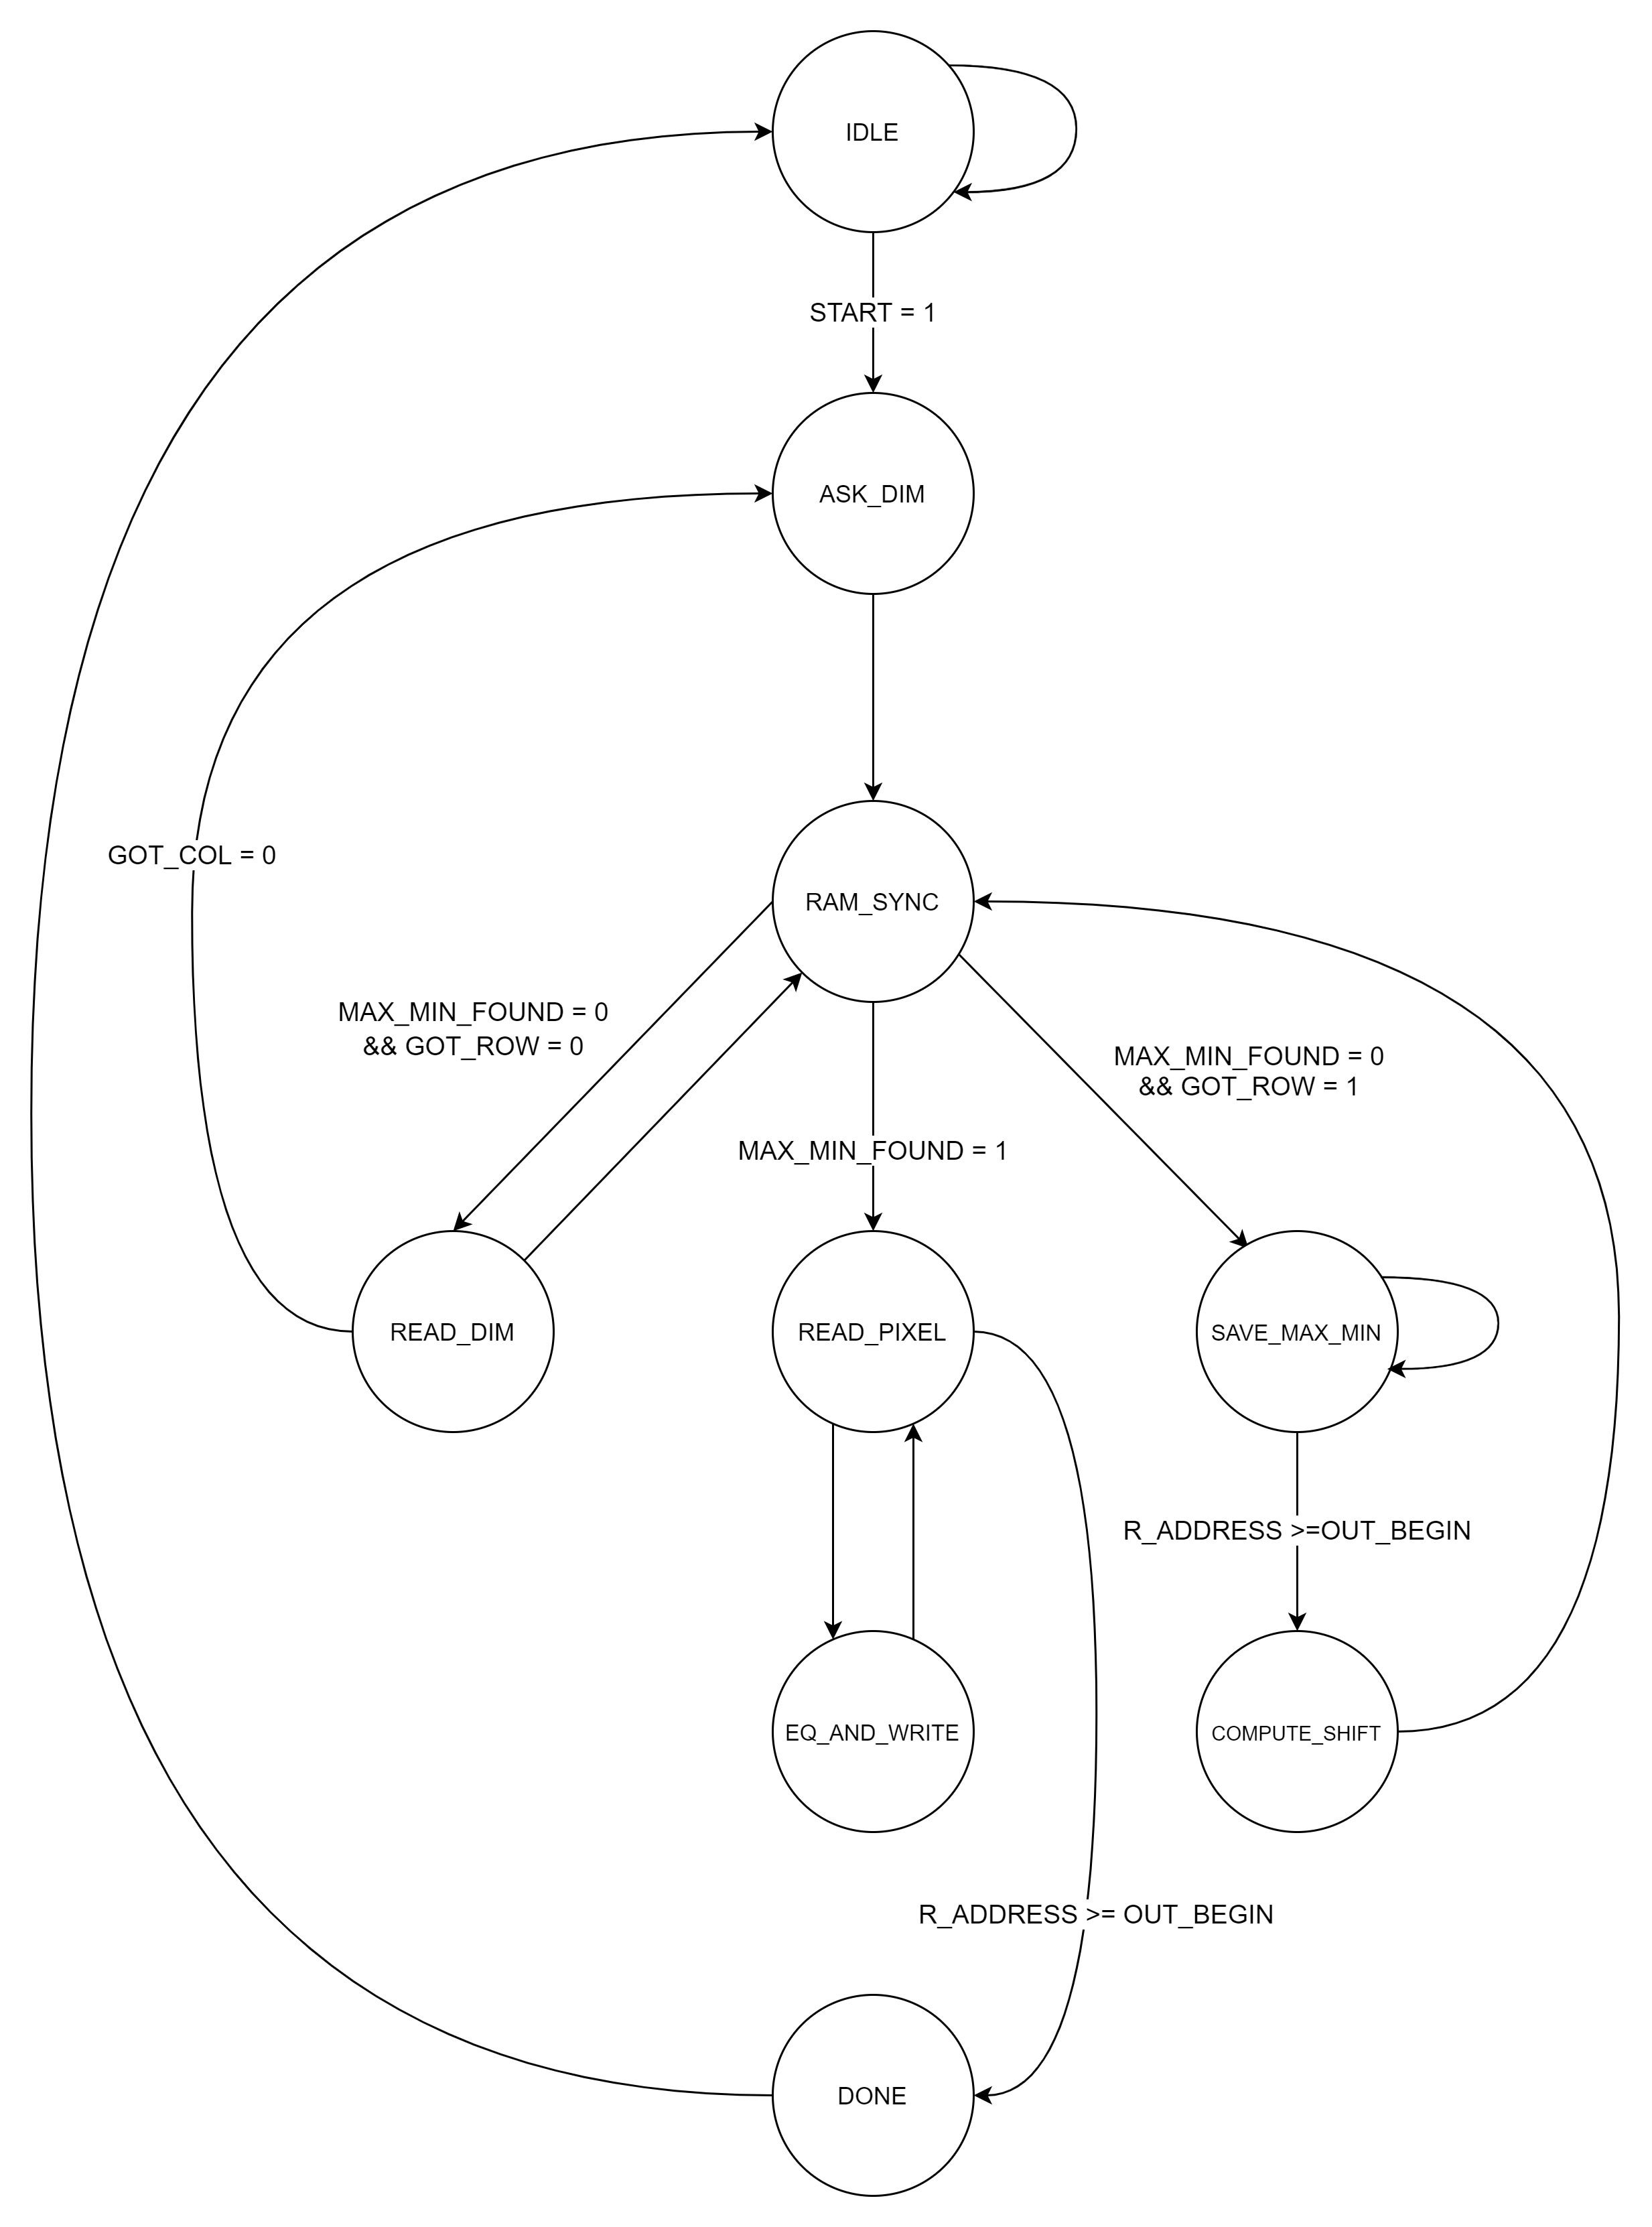
\includegraphics[scale=0.150]{architettura/FSM diagram.png}
    \caption{Diagramma degli stati del dispositivo}
    \label{fig:fsm_diagram}
\end{figure}


\pagebreak
\subsection{Descrizione degli stati}
Di seguito è riportata una breve descrizione di ogni stato.

\subsubsection{IDLE}
Stato iniziale, in cui si attende il segnale di START. \\
Non appena tale segnale è ricevuto, parte del dispositivo viene reinizializzata in modo da permettere di processare più immagini senza un segnale di RESET. \\
Inoltre si ritorna a questo stato quando viene ricevuto il segnale di RESET.
\subsubsection{ASK\_DIM}
Stato in cui viene richiesto alla memoria il numero di colonne dell'immagine (N\_COL), oppure il numero di righe (N\_ROW) in caso quest'ultimo sia già stato salvato.
\subsubsection{RAM\_SYNC}
In questo stato sono condensate tutte le possibili situazioni di attesa in seguito alla richiesta di un dato alla memoria. \\
Inoltre, esso è in grado di richiedere un dato alla memoria, in modo da minimizzare i cicli di clock passati in attesa.
\subsubsection{READ\_DIM}
In questo stato vengono letti da memoria i valori corrispondenti al numero di colonne e al numero di righe dell'immagine. \\
Inoltre viene calcolato l'indirizzo del primo byte di memoria in cui salvare l'immagine equalizzata, chiamato OUT\_BEGIN
\subsubsection{SAVE\_MAX\_MIN}
Stato in cui viene letta la memoria fino a quando l'indirizzo di lettura non corrisponde a OUT\_BEGIN.
In questo stato vengono salvati il massimo e il minimo valore dei pixel dell'immagine: MAX\_VALUE e MIN\_VALUE
\subsubsection{COMPUTE\_SHIFT}
Stato in cui viene eseguita la prima parte dell'algoritmo di equalizzazione, ossia quella che non dipende da CURRENT\_PIXEL. \\
Viene calcolato DELTA\_VALUE e si ricava SHIFT\_LEVEL discretizzando tramite dei controlli a soglia.
\subsubsection{READ\_PIXEL}
In questo stato viene salvato temporaneamente in memoria il valore del pixel dell'immagine che si sta processando. \\
La lettura dell'immagine procede fino a quando l'indirizzo di lettura non corrisponde a OUT\_BEGIN, in tal caso l'algoritmo è stato completato e il componente passa allo stato DONE.
\subsubsection{EQ\_AND\_WRITE}
In questo stato viene eseguita la seconda parte dell'algoritmo di equalizzazione, ossia quella che dipende da CURRENT\_PIXEL. \\
Vengono calcolati TEMP\_PIXEL e NEW\_PIXEL.
Infine viene richiesta alla memoria la scrittura di NEW\_PIXEL al ciclo di clock successivo.
\subsubsection{DONE}
Stato finale, in cui si attende che il segnale START venga abbassato, per poi tornare nello stato IDLE. 

\newpage
\section{Risultati sperimentali}
\subsection{Report di sintesi}
Tool di sintesi: Vivado WebPack 2021.1 \\
FPGA target: Artix-7 xc7a200tfbg484-1 

Di seguito sono riportati gli elementi più significativi del report di utilizzo di Vivado:

\begin{table}[h]
    \centering
    \begin{tabu*} to 1.0\textwidth { |X[1c]|X[0.6c]|X[0.6c]|X[0.6c]|}\hline
        \rule[3ex]{0pt}{0.5ex} \textbf{Componente} & \textbf{Usati} & \textbf{Disponibili} & \textbf{\% Utilizzo}\\\hline
        \rule[3ex]{0pt}{0.5ex} LUT as Logic & 204 & 134600 & 0.15 \\\hline
        \rule[3ex]{0pt}{0.5ex} LUT as Memory & 0 & 46200 & 0.00 \\\hline
        \rule[3ex]{0pt}{0.5ex} Register as Flip Flop & 118 & 269200 & 0.04 \\\hline
        \rule[3ex]{0pt}{0.5ex} Register as Latch & 0 & 269200 & 0.00 \\\hline
        \rule[3ex]{0pt}{0.5ex} F7 Muxes  & 1 & 67300 & \verb|<|0.01 \\\hline
        \rule[3ex]{0pt}{0.5ex} F8 Muxes  & 0 & 33650 & 0.00 \\\hline
        \rule[3ex]{0pt}{0.5ex} I/O Buffer & 38 & 285 & 13.33 \\\hline
    \end{tabu*}
\end{table}

Di seguito sono riportati altri valori significativi estratti dal report generale:

\begin{table}[h]
    \centering
    \begin{tabu*} to 1.0\textwidth { |X[1c]|X[0.6c]|X[2c]|}\hline
        \rule[3ex]{0pt}{0.5ex} \textbf{Descrizione} & \textbf{Valore} & \textbf{Note} \\\hline
        \rule[3ex]{0pt}{0.5ex} Data Path Delay &  8.157 ns & Logic=4.184 ns, Route=3.973 ns \\\hline
        \rule[3ex]{0pt}{0.5ex} Total On-Chip Power & 5.039 W & Dynamic=4.885 W, Device Static=0.154 W  \\\hline
        \rule[3ex]{0pt}{0.5ex} Livelli logici & 11 & \footnotesize{CARRY4=6, IBUF=1, LUT2=1, LUT4=1, LUT6=2} \\\hline
        \rule[3ex]{0pt}{0.5ex} Schematic Nets & 659 &  \\\hline
        \rule[3ex]{0pt}{0.5ex} Schematic Cells & 470 &  \\\hline
    \end{tabu*}
\end{table}

\subsection{Simulazioni}
I seguenti test sono stati eseguiti sia in pre-sintesi (Behavioral Simulation) che in post-sintesi (Post-Synthesis Functional Simulation).\\
Tutti i test sono stati superati in entrambi i casi, tuttavia per maggiore chiarezza gli screenshot mostrati in questa sezione provengono tutti da simulazioni pre-sintesi.

\subsubsection{Test con analisi dettagliata}
Per rendere più chiaro il funzionamento del dispositivo, di seguito è riportata l'analisi step-by-step di una simulazione, per brevità con in input un'immagine di dimensione 2x2.

\subsubsection*{START e lettura dimensioni}

\begin{figure}[h]
    \centering
    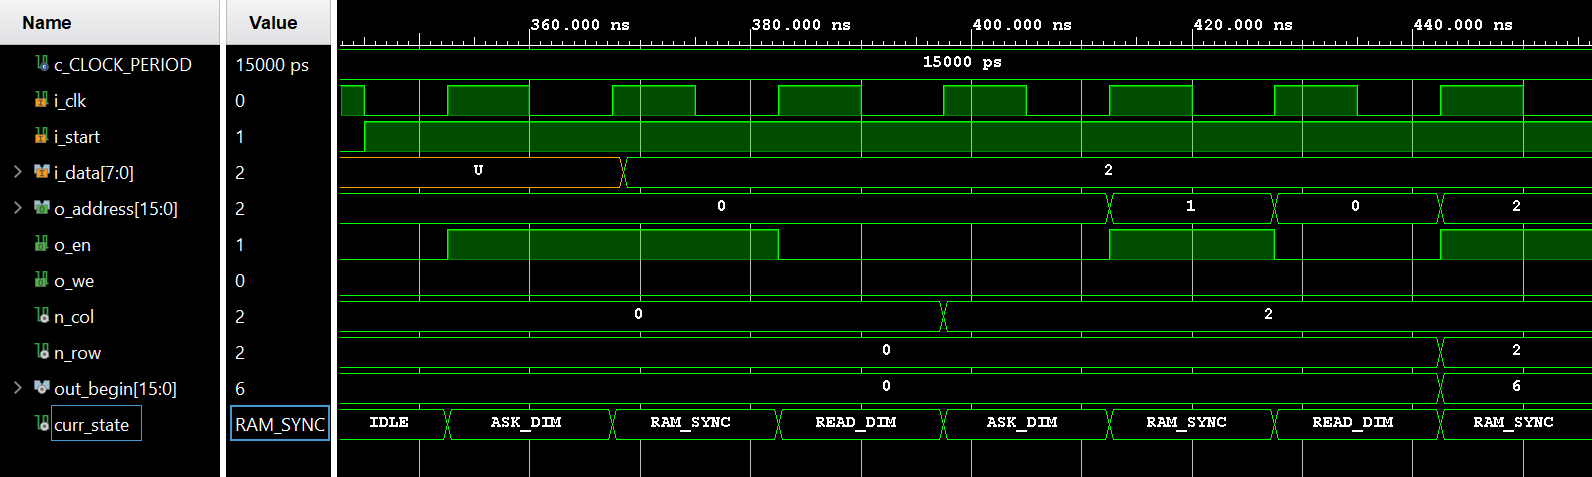
\includegraphics[trim=0cm 1.25cm 0cm 0.25cm, width=1.0\textwidth]{simulazioni/2x2_SRD.png}
    \label{fig:2x2_SRD}
\end{figure}
Come evidenziato dallo screenshot, non appena viene ricevuto START = 1, il dispositivo passa allo stato ASK\_DIM e richiede alla memoria il byte all'indirizzo 0, ossia la dimensione delle colonne. 
Dopo aver atteso un ciclo di clock per assicurarsi della stabilità del valore presente in memoria (stato RAM\_SYNC), il dato richiesto è letto e salvato nello stato READ\_DIM. \\
In seguito si ripete tale procedimento per il byte all'indirizzo 1, ossia la dimensione delle righe.
Subito dopo la lettura di tale valore è calcolato il valore di OUT\_BEGIN. 
Infine il dispositivo si porta nuovamente nello stato RAM\_SYNC, settando O\_ADDRESS = 2 per segnalare alla memoria di voler iniziare la lettura dei pixel dell'immagine

\subsubsection*{Calcolo MAX, MIN e SHIFT\_LEVEL}
\begin{figure}[h]
    \centering
    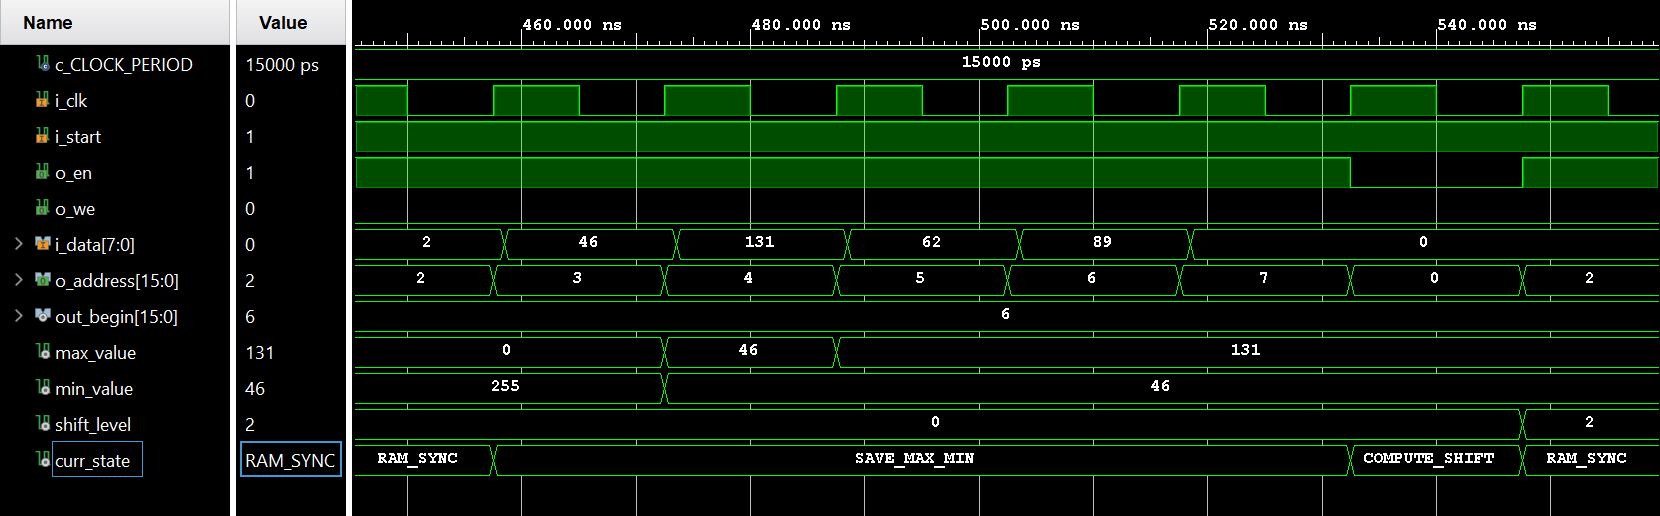
\includegraphics[trim=0cm 1.25cm 0cm 0.25cm, width=1\textwidth]{simulazioni/2x2_MMSL.png}
    \label{fig:2x2_MMSL}
\end{figure}
In questa fase l'immagine è letta sequenzialmente, un pixel per ogni ciclo di clock. \\
Lo screenshot mostra chiaramente come, nello stato SAVE\_MAX\_MIN, MAX\_VALUE e MIN\_VALUE siano aggiornati o meno in base alla lettura del pixel corrente. Si passa allo stato seguente  quando il valore di O\_ADDRESS diventa maggiore del valore di OUT\_BEGIN. In questo stato (COMPUTE\_SHIFT) viene calcolato SHIFT\_LEVEL. \\
Anche in questo caso il dispositivo si riporta poi nello stato RAM\_SYNC, segnalando di necessitare di un'altra lettura dell'immagine per equalizzarla.

\vspace{3cm}
\subsubsection*{Equalizzazione, write e DONE}
\begin{figure}[h]
    \centering
    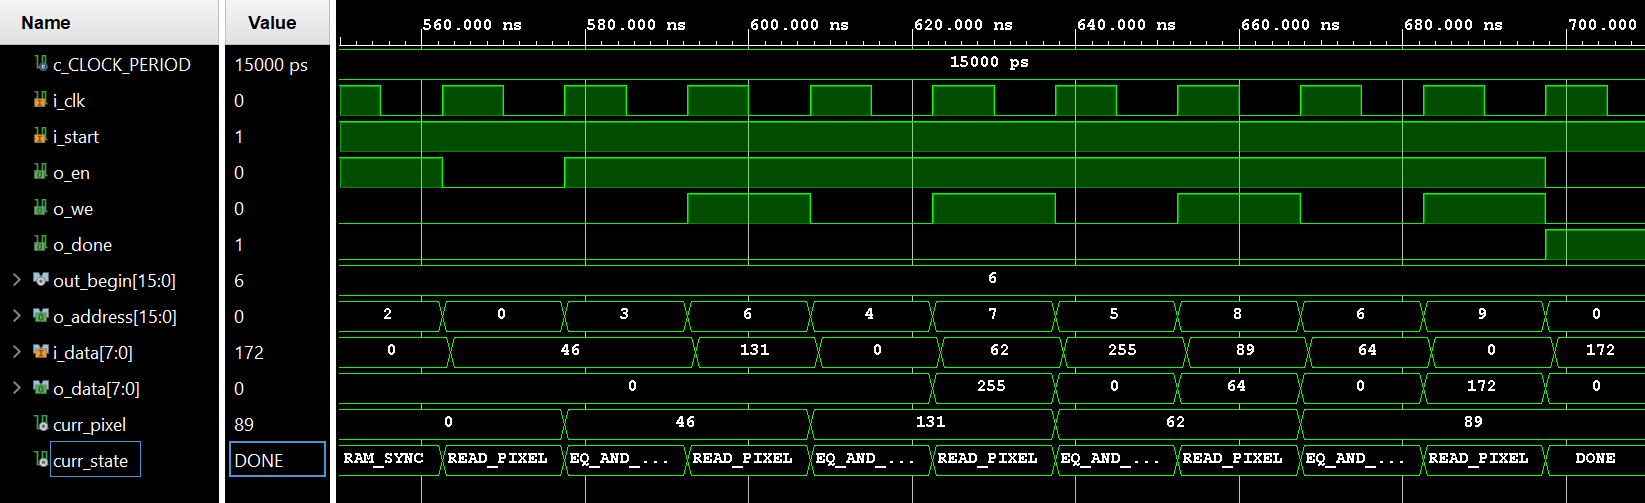
\includegraphics[trim=0cm 1.25cm 0cm 0.25cm, width=1\textwidth]{simulazioni/2x2_EWD.png}
    \label{fig:2x2_EWD}
\end{figure}
In questa fase avviene, sequenzialmente e pixel per pixel, la lettura del valore di un pixel e la scrittura del suo corrispondente valore equalizzato. \\
Nello stato READ\_PIXEL viene letto il valore del pixel originale e salvato temporaneamente in CURR\_PIXEL. Nello stato EQ\_AND\_WRITE si esegue l'equalizzazione partendo da tale valore e in seguito si richiede alla memoria la scrittura del valore equalizzato nel rispettivo indirizzo. \\
Gli stati READ\_PIXEL e EQ\_AND\_WRITE si alternano fino a quando la lettura in READ\_PIXEL non arriva al valore di OUT\_BEGIN: in tal caso l'algoritmo è terminato e il dispositivo passa allo stato DONE, portando il segnale \textbf{o\_done} a 1. \\
Infine il dispositivo torna allo stato IDLE, pronto per ricevere un altro segnale di START.

\bigskip
\subsubsection{Test dei casi limite}
Per prima cosa sono stati testati i casi limite, usando degli appositi TestBench.\\
Ne sono stati individuati 5:
\paragraph*{Immagine di dimensione 0x0:}
poiché non è presente alcuna immagine in memoria, come previsto l'esecuzione termina senza processare alcun pixel e senza modificare in alcun modo la memoria.
\paragraph*{Immagine di dimensione 1x1:}
poiché vi è un unico pixel, a prescindere dal suo valore avremo CURRENT\_PIXEL\_VALUE - MIN\_PIXEL\_VALUE = 0, che forza tutti i pixel in uscita al valore 0. Di conseguenza l'esecuzione termina eseguendo una sola scrittura all'indirizzo 3 della memoria, come previsto.
\paragraph*{Immagine di dimensione 128x128:}
la simulazione termina correttamente, modificando la memoria nel modo previsto.\\
Questo TestBench permette di assicurarsi dell'assenza di problemi dovuti a un errato dimensionamento di segnali e/o variabili, e dunque di registri in post-sintesi.
\paragraph*{Immagine con tutti i pixel a 0:}
poiché tutti i pixel hanno lo stesso valore, si verifica nuovamente che CURRENT\_PIXEL\_VALUE - MIN\_PIXEL\_VALUE = 0. Il dispositivo termina l'esecuzione scrivendo in memoria soltanto pixel dal valore 0.
\paragraph*{Immagine con tutti i pixel a 255:}
come nel caso precedente, sempre perché tutti i pixel hanno lo stesso valore. 

\subsubsection{Immagini in sequenza con RESET}
\begin{figure}[h]
    \centering
    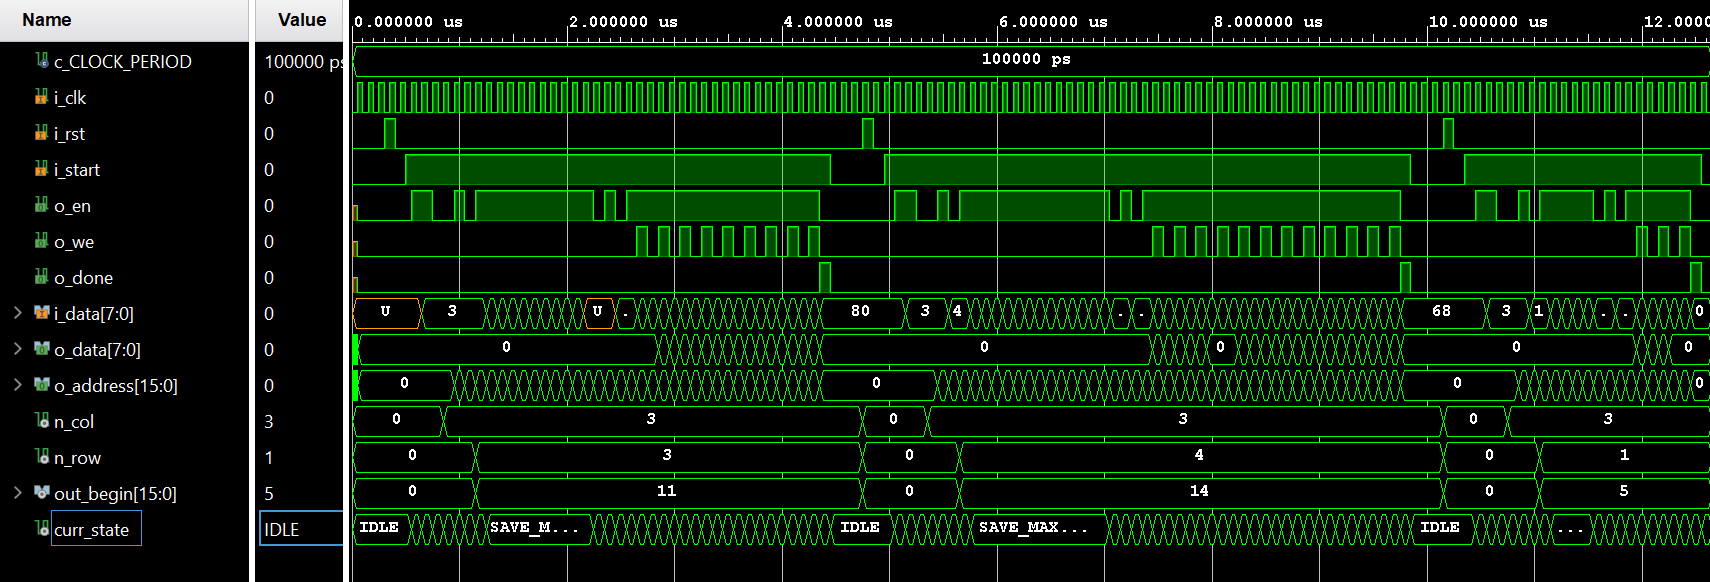
\includegraphics[trim=0cm 1.25cm 0cm 0.25cm, width=1.0\textwidth]{simulazioni/GEN_RESET.png}
    \label{fig:gen_reset}
\end{figure}
In questo test è richiesto al dispositivo di processare più immagini in sequenza (in questo caso 3) e tra ogni immagine e la successiva viene nuovamente inviato il segnale di RESET. \\
Il test evidenzia come il RESET del dispositivo funzioni correttamente, in quanto ogni computazione termina correttamente. Inoltre, dallo screenshot è possibile osservare come il segnale di RESET causi la reinizializzazione dei segnali (come \textbf{n\_col}, \textbf{ n\_row} e \textbf{out\_begin}). \\
Da notare che sono stati eseguiti altri test sulla falsa riga di quest'ultimo, con più immagini e di dimensioni maggiori.

\subsubsection{Immagini in sequenza senza RESET}
\begin{figure}[h]
    \centering
    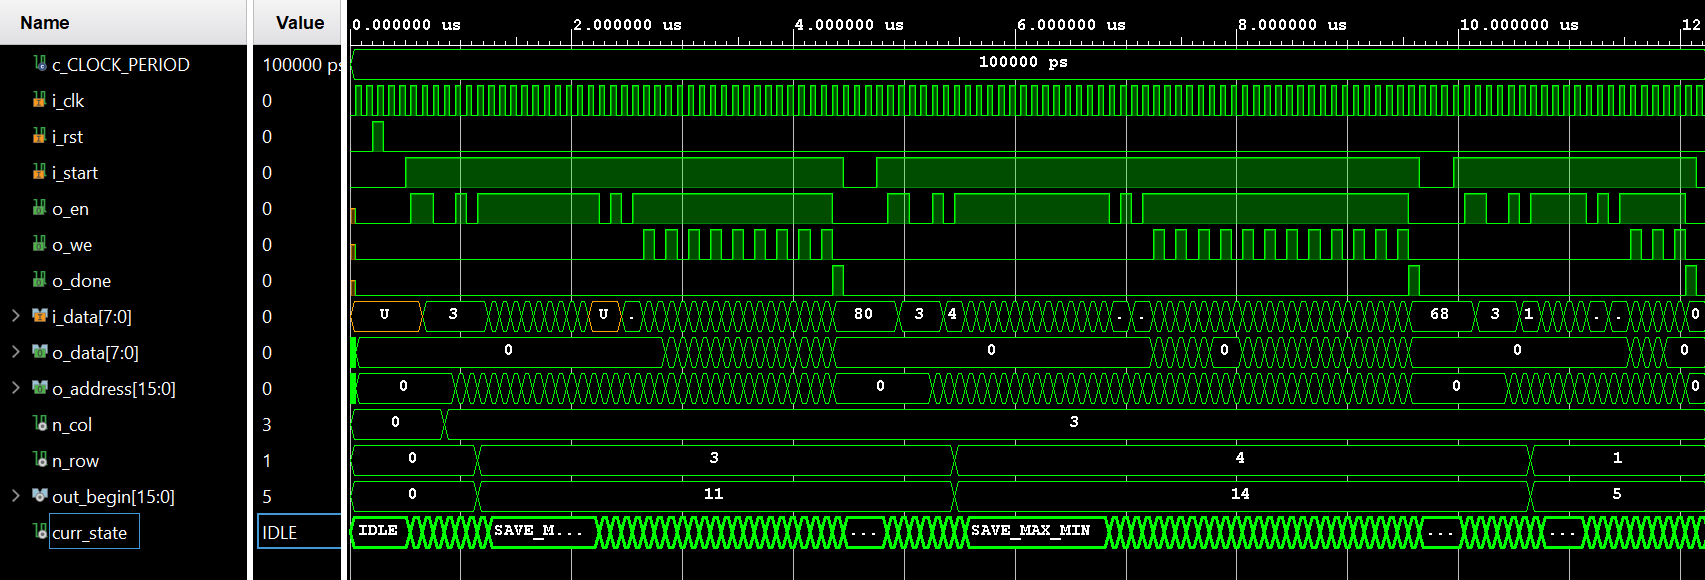
\includegraphics[trim=0cm 1.25cm 0cm 0.25cm, width=1.0\textwidth]{simulazioni/GEN_NO_RESET.png}
    \label{fig:gen_no_reset}
\end{figure}
L'unica differenza tra questo test e il precedente è appunto l'utilizzo del segnale di  RESET: in questo caso viene inviato solo a inizio simulazione e non anche tra un'immagine e la successiva. \\
Anche in questo caso tutte le simulazioni terminano correttamente, in quanto una nuova ricezione del segnale di START causa una reinizializzazione parziale del dispositivo. \\
Questo test evidenzia la correttezza della relazione tra i segnali i\_start e o\_done: come richiesto da specifica, il segnale DONE è portato ad alto solo dopo la fine dell'elaborazione e rimane alto fino a che il segnale di START non è riportato a 0.

\subsubsection{Test generici}
Infine ci si è voluti assicurare del corretto comportamento del dispositivo mediante altri numerosi test che non vanno a verificare casi particolari ma utilizzano dati qualsiasi il più possibile differenziati. Tali test, qui non riportati per brevità, terminano tutti fornendo il risultato atteso.

\newpage
\section{Conclusioni}
In base al report di sintesi e ai risultati delle simulazioni, si può affermare che il componente progettato:
\begin{itemize}
    \item Rispetta la specifica
    \item Funziona correttamente in pre-sintesi
    \item Risulta correttamente sintetizzabile
    \item Funziona correttamente in post-sintesi
\end{itemize}
Inoltre, sono stati raggiunti gli obiettivi prefissati, ottenendo un numero di stati ridotto e garantendo una gestione efficiente della memoria senza compromettere la leggibilità e la chiarezza di codice sorgente e diagramma degli stati.
\end{document}